\chapter{持有股票的同时买入看跌期权\label{CH17}}
\section{买什么样的看跌期权}
股票持有者选择应当买什么样的看跌期权,决定了他要放弃多少潜在盈利以及限制多大的风险。虚值看跌期权的成本很小。因此,如果标的股票价格上涨,它对潜在盈利就只是较小的障碍。不幸的是,这样的看跌期权在股票价格跌到期权行权价之前的保护功能也小。因此,买入虚值看跌期权所提供的下行方向的保护没有买入实值期权那么大。买入深度虚值期权作为保护更像是一种“灾难保险”:如果在这个看跌期权的存续期内股票出现灾难性暴跌,股票持有者可以从这样的看跌期权中得到保护,但是,如果股票下跌有限,它就提供不了什么保护。

另一方面,股票持有者可以买入一手实值看跌期权作为保护。这样会严重限制他的潜在盈利,因为标的股票必须上涨到比行权价更高的地方,他才有盈利可言。不过,实值看跌期权在下行方向提供了巨大的保护,将他的亏损限制到非常小的数量。

\begin{tcolorbox}
    XYZ 的价格同样是 40,10 月 45 看跌期权的售价为 5.50 点。买入 10 月 45 看跌期权的股票持有者的最大风险是 0.50 点,因为在任何时候都可以将这个看跌期权行权,按 45 的价格卖掉股票,这样在股票上就会有 5 点的收益。他为这手看跌期权付了 5.50 点,所以他总的最大亏损是 0.50 点。但是,在这个看跌期权的存续期里,他很难从这个头寸中盈利,在 10 月到期时他想要有任何盈利,XYZ 就必须上涨 5.50(看跌期权的成本)以上。
\end{tcolorbox}

买入深度实值的看跌期权是一个过度保守的策略,因而通常不是一个好策略。另一方面,买入深度虚值的看跌期权也不是一种聪明的做法。\textcolor{red}{一般来说,交易者应当买入略为虚值的看跌期权作为保护}。这样就可以在对保护股票的正面作用和限制盈利的负面作用之间达到一种平衡。
\section{买入看跌期权作为对备兑看涨期权卖出者的保护}
因为买入看跌期权为普通股股票的持有者提供了保护,有的投资者自然会想到,同样的保护特性也可以用来限制他们在卖出备兑看涨期权策略中的下行风险。卖出备兑看涨期权涉及买入股票和就股票卖出一手看涨期权。卖出备兑在上行方向的潜在盈利有限,在下行方向提供了同看涨期权权利金数量相等的保护。如果股票价格在到期时稍许下跌、保持不变或者上涨,备兑卖出者就能盈利。当股票下跌的幅度超过所收入的看涨期权权利金时,备兑卖出者才会实际亏损。他在下行方向有很大的潜在风险。整个策略被称为保护性领圈(protective collar),或者简称为“领圈”(collar)。

买入虚值看跌期权可以为卖出备兑消除大的潜在亏损,但花在买入看跌期权上的钱会减少这手卖出备兑的总收益。因此,交易者在决定是否值得买入这手看跌期权时,必须将它的成本包括在最初的计算中。

% \begin{figure}
%     \centering
%     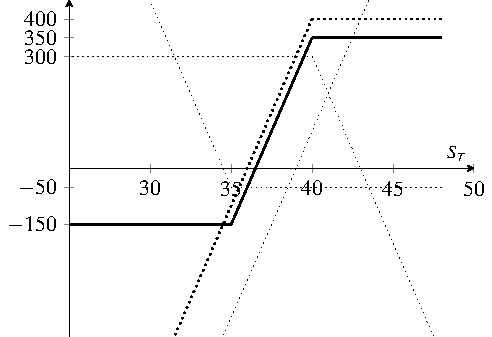
\includegraphics[width=0.8\textwidth]{../IMG/accumulator.pdf}
%     \caption{买入看跌期权保护的卖出备兑看涨期权}
%     \label{fig:covered call with long put}
% \end{figure}

没有保护性看跌期权的备兑卖出者为了得到更大的下行方向的保护,就不得不向下挪仓。向下挪仓意味着买回目前卖出的那手看涨期权,再卖出另一手行权价较低的看涨期权来代替它。如果股票在下跌之后价格稳定下来,那么,向下挪仓的做法会有帮助。可是,如果股票反转过来,价格重新上升,那么,因为向下挪仓,备兑卖出者的盈利就受到限制。事实上,他甚至可能“锁定”了一笔亏损。有保护性看跌期权的备兑卖出者就不需要操心这种事。他永远不需要向下挪仓,因为他的最大亏损是有限的。因此,他永远不会落入“锁定”亏损的局面。这是一个很大的优势,特别是从情绪的角度来看,因为卖出者永远也不会被迫在股票价格下跌的过程中对股票价格的未来走向做出判断。有了这个看跌期权,他就完全可以不采取任何行动,因为他总的亏损是有限的。如果股票价格后来反弹,他仍然可以获得最大盈利。

\section{无成本领圈}
“领圈”策略往往是以另一种形式出现:一个股票持有者开始对股市会下跌的可能性感到担心,决定要就他的股票买入看跌期权作为保护。但是,看跌期权的成本使他感到沮丧,因此,他同时也考虑要卖出看涨期权。如果他买入一手虚值看跌期权,那么,很有可能他可以卖出一手看涨期权,其收入可以完全抵消这手虚值看跌期权的成本。因此,他就不用成本就能建立起一手保护性领圈,至少没有支出。\textbf{他的“成本”是放弃了股票在卖出的看涨期权的行权价之上的潜在盈利。}

因此,交易者在建立领圈时,即使他不是一个机构交易者,也应当考虑使用长期期权(LEAPS),因为这样的看涨期权的行权价同看跌期权的行权价相比或者同标的股票的价格相比,会高出许多。
\paragraph{使用较低行权价进行部分卖出备兑}
应当指出,交易者不一定要完全放弃他股票中的全部潜在盈利。他可以像往常一样买入看跌期权,然后卖出行权价比一手低成本的领圈所需要的稍低一些的看涨期权,但卖出的看涨期权的数量要少于所持有的股票的数量。这样做,在标的股票的一些股份上就会有无限的潜在盈利。
\section{调整领圈}
如果标的股票价格急剧下降,领圈可能会有所调整。股价下跌以后,看跌期权的价值比较大,而看涨期权的价值则很小。如果投资者认股票已经跌得差不多了时,他只会卖出看跌。至于他是要覆盖看涨期权,如果股价反弹,投资者将有有很大的盈利潜力。在另一方面,如果投资者不确定股票是否不会再跌,他可能只周转看跌期权,或者看跌期权和看涨期权一起,到低于行权价格,因此从头寸中获得很大的应收(应收来自于出售原看跌期权,这目前是非常有价值的)。作为第三选择,他也会考虑对他拥有的看跌期权售出一些虚值看跌期权。这会带来一些应收,但会导致股票在低于卖出的看跌期权的行权价时有亏损。

在另一方面,如果在领圈建立之后标的股票价格大幅增加,唯一退出领圈的方法是覆盖卖出的看涨期权,这将生成(很大的)应付。当然,标的股票的价格上涨,所以这是一个可以用来抵消看涨期权亏损的未实现利润。本质上,不存在从上面退出领圈的方便的策略。

总的来说,在使用“领圈”的策略上,交易者可以富有创造性。有一件事需要记住:\textbf{如果交易者不想卖掉他持有的股票,那么,在他的头脑里,他实际上是在卖出裸看涨期权。}也就是说,如果交易者持有“不能”卖的股票,这或许是因为卖掉股票后的灾难性税务负担,或者是因为这个股票在“家族里”已经有了很长时间。那么,他就不应当就它而卖出备兑看涨期权,因为他将不得不把这个看涨期权作为裸期权来处理(如果他拒绝卖掉股票的话)。如果股票价格大幅上涨,这就会造成相当大的惊恐,要是一开始就避免在这个股票上卖出看涨期权,那么,就可以很容易地免除这种恐慌。